\documentclass[compress,xcolor=table]{beamer}

\usepackage[french]{babel}
\selectlanguage{french}
\usepackage[utf8]{inputenc}
\usepackage[T1]{fontenc}
\usepackage{tikz}
\usepackage{wrapfig}
\usepackage{multirow}
\usepackage{pgf-pie}
\usepackage{pgfplots}
\usepackage{pdfpages}
\usepackage{vocabulaireEpicUnityPresentation}
\usepackage{commun/vocabulaireCommun}
\usepackage{hyperref}
\usepackage{movie15}

\usetheme{eastpic}

% code pour pouvoir mettre des cellcolor qui dépendent de la frame...
\makeatletter
\def\rowcolor{\noalign{\ifnum0=`}\fi\bmr@rowcolor}
\newcommand<>{\bmr@rowcolor}{%
    \alt#1%
	{\global\let\CT@do@color\CT@@do@color\@ifnextchar[\CT@rowa\CT@rowb}% 
	{\ifnum0=`{\fi}\@gooble@rowcolor}% 
}

\newcommand{\@gooble@rowcolor}[2][]{\@gooble@rowcolor@}
\newcommand{\@gooble@rowcolor@}[1][]{\@gooble@rowcolor@@}
\newcommand{\@gooble@rowcolor@@}[1][]{\ignorespaces}
\makeatother



\makeatletter
\def\cellcolor{{\ifnum0=`}\fi\bmr@cellcolor}
\newcommand<>{\bmr@cellcolor}{%
    \alt#1%
	{\global\let\CT@do@color\CT@@do@color\@ifnextchar[\CT@rowa\CT@rowb}%
	 {\ifnum0=`{\fi}\@gooble@cellcolor}%
}

\newcommand{\@gooble@cellcolor}[2][]{\@gooble@cellcolor@}
\newcommand{\@gooble@cellcolor@}[1][]{\@gooble@cellcolor@@}
\newcommand{\@gooble@cellcolor@@}[1][]{\ignorespaces}

\newcommand{\tablenameUn}{Tableau 1 : Temps de conversion en fonction du nombre de fiches}



\def\sectionintoc{}
\def\beamer@sectionintoc#1#2#3#4#5{%
\ifnum\c@tocdepth>0%
\ifnum#4=\beamer@showpartnumber%
{
  \beamer@saveanother%
  \gdef\beamer@todo{}%
  \beamer@slideinframe=#1\relax%
  \expandafter\only\beamer@tocsections{\gdef\beamer@todo{%
      \beamer@tempcount=#5\relax%
      \advance\beamer@tempcount by\beamer@sectionadjust%
      \edef\inserttocsectionnumber{\the\beamer@tempcount}%
      \def\inserttocsection{\hyperlink{Navigation#3}{#2}}%
      \beamer@tocifnothide{\ifnum\c@section=#1\beamer@toc@cs\else\beamer@toc@os\fi}%
      {
        \ifbeamer@pausesections\pause\fi%
        \ifx\beamer@toc@ooss\beamer@hidetext
          \vskip1em
        \else
          \vfill
        \fi
        {%
          \hbox{\vbox{%
              \def\beamer@breakhere{\\}%
              \beamer@tocact{\ifnum\c@section=#1\beamer@toc@cs\else\beamer@toc@os\fi}    {section in toc}}}%
         \par%
        }%
      }%
    }
  }%
  \beamer@restoreanother%
  }
  \beamer@todo%
  \fi\fi%
}



\makeatother
% end code pour pouvoir mettre des cellcolor qui dépendent de la frame


\title{Présentation de projet EDTS}
\date{\today}
\author{Zhaolun Wang et Zenan Xu}
\institute{\insa}

\setbeameroption{show notes}

\begin{document}


\begin{frame}[plain]
	\titlepage
\end{frame}

\begin{frame}{Sommaire}
	\tableofcontents[hideallsubsections]
\end{frame}

\section[Introduction]{Introduction}
\subsection{}

%\begin{frame}{Le client, Fondation UNIT}

\begin{figure}
\centering
\includegraphics[width=5cm]{images/logo.png}
\caption{Logo de la fondation UNIT}
\end{figure}

\begin{itemize}
  \pause
  \item UNIT: l'Université Numérique Ingénierie et Technologie ;
  \pause
  \item Fondation partenariale d'environ 70 Universités, Grandes Ecoles d'Ingénieurs et Entreprises ;
  \pause
  \item Une des sept universités numériques thématiques (UNT) nationales.

\end{itemize}
	
\end{frame}

\begin{frame}{L'équipe \textsc{EpicUnity}}
	
	\begin{figure}
	\centering
	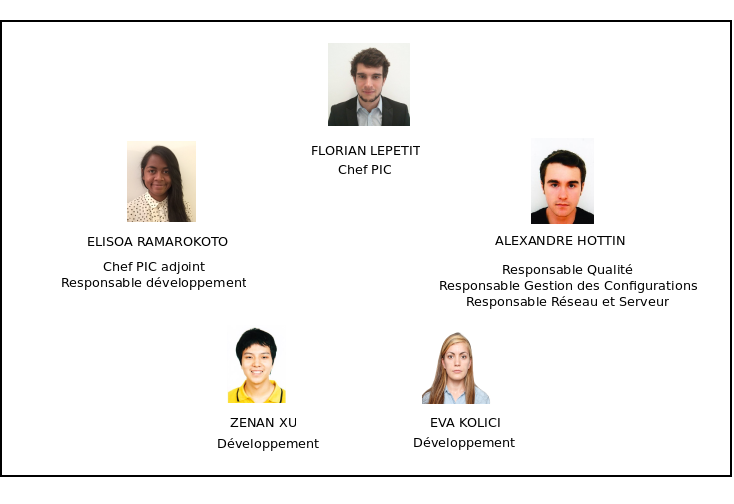
\includegraphics[width=10cm]{images/organigramme.png}
	\caption{Organigramme de l'équipe}
	\end{figure}
	
\end{frame}



\section[Objectifs]{Objectifs du projet}
\subsection{}
%\speaker{\Eva{}}
\begin{frame}{Situation du client}
	\begin{itemize}
	  \item 1200 ressources propres à UNIT + 2800 autres ressources sur les serveurs des partenaires;
	  \item ORI-OAI : serveur de stockage;
	  \item Projet SEMUNIT en 2010 de Madame Yolaine Bourda.
	\end{itemize}
\end{frame}

\begin{frame}{Demandes principales du client}

\begin{itemize}
	  \item Formation aux technologies du Web Sémantique ;
	  \item Reprise du modèle prototype SEMUNIT;
	  \item Obtention d'une base RDF interrogeable en SPARQL automatiquement mise à jour;
	  \item Développement d'une application utilisant la base RDF précédente permettant de cartographier les ressources des établissements.
	\end{itemize}
  
\end{frame}


\begin{frame}{Problématiques et besoins}
	\begin{figure}
	  \centering
	  \includegraphics[width=9cm]{images/exemple.pdf}
	  \caption{Exemple d'une problématique simple}
	\end{figure}
	
\end{frame}

\speaker{\Alexandre{}}
\begin{frame}{Solution -  Web Sémantique}
	\begin{figure}
	  \centering
	  \includegraphics[width=6.5cm]{images/pyramide.pdf}
	  \caption{Pyramide du Web}
	\end{figure}
	
\end{frame}


\begin{frame}{Solution - Web Sémantique}
	\begin{figure}
	  \centering
	  \includegraphics[width=6cm]{images/pile.pdf}
	  \caption{Pile de standardisation - Nicolas Delestre}
	\end{figure}
\end{frame}

\speaker{\Eva{}}


\begin{frame}{Architecture globale du projet}

	
	\begin{figure}
	  \centering
	  \includegraphics[width=10cm]{images/objectifs.pdf}
	  \caption{Schéma explicatif du sujet de ce semestre}
	\end{figure}

\end{frame}


\section[Prérequis]{Prérequis technologique}
\subsection{}
%\speaker{\Zenan{}}

\begin{frame}{Profil d'application}
	\begin{figure}
	  \centering
	  \includegraphics[width=10cm]{images/Historique_suplomfr.png}
	  \caption{Historique du profil d'application SupLOMFR\footnotemark}
	\end{figure}
	\footnotetext{Source : http://www.sup.lomfr.fr/}
\end{frame}


\speaker{\Quentin{}}

\begin{frame}{Conceptualisation}
\begin{figure}


	  \begin{overprint}

	 \onslide<1>\centerline{\includegraphics[width=8cm]{images/pilepart.pdf}}
	 \onslide<2>\centerline{\includegraphics[width=8cm]{images/pilepart1.pdf}}
	 \onslide<3>\centerline{\includegraphics[width=8cm]{images/pilepart2.pdf}}
	 \onslide<4>\centerline{\includegraphics[width=8cm]{images/pilepart3.pdf}}
	 \onslide<5>\centerline{\includegraphics[width=8cm]{images/pilepart4.pdf}}

	  \end{overprint}
	  \caption{Pile de standardisation}
	  
\end{figure}
\end{frame}

\begin{frame}{RDF (Représentation)}
\begin{figure}
	  \centering
	  \includegraphics[width=10cm]{images/RdfExemple.pdf}
	  \caption{triplets RDF}
\end{figure}
\pause

- \textbf{DataProperty} \newline
- \textbf{ObjectProperty}

\pause

\begin{figure}
	  \centering
	  \includegraphics[width=10cm]{images/RdfCode.png}
	  \caption{Exemple RDF}
\end{figure}
\end{frame}
\begin{frame}{RDFS - OWL (Raisonnement)}
\begin{figure}
	  \centering
	  \includegraphics[width=11.5cm]{images/RdfsExemple.pdf}
	  \caption{Exemple RDFS}
\end{figure}
\pause
\begin{figure}
	  \centering
	  \includegraphics[width=11.5cm]{images/OwlExemple.pdf}
	  \caption{Exemple OWL}
\end{figure}
\end{frame}

\begin{frame}{SKOS (Vocabulaire spécifique)}

Choix de SKOS : \textbf{Vocabulaire spécifique} + \textbf{Alignement ontologique}

% Please add the following required packages to your document preamble:
% \usepackage{multirow}
\begin{table}[h]
\begin{tabular}{|l|l|l|}
\hline
Cycle CanCore     & Années cumulées & Cycle SupLOMFR \\ \hline
\multirow{4}{*}{} & 13              & Baccalauréat   \\ \cline{2-3} 
  Baccalauréat  & 14              & Licence 1      \\ \cline{2-3} 
                  & 15              & Licence 2      \\ \cline{2-3} 
                  & 16              & Licence 3      \\ \hline
\end{tabular}
\end{table}

\end{frame}

\begin{frame}{Représentation de type UML}
\begin{figure}
	  \centering
	  \includegraphics[width=8cm]{images/UML_class.pdf}
	  \caption{Notre choix de représentation UML}
	  % EXPLICATION DATA OBJECT PROPERTY
\end{figure}
\end{frame}

% \begin{frame}{Représentation de type UML}
% \begin{figure}
%   \begin{minipage}[c]{.24\linewidth}
% 	  \centering
% 	  \includegraphics[width=3cm]{images/UML_class_categorie9.pdf}
% 	  \caption{Représentation en type UML de la catégorie 9}
%   \end{minipage} \hfill
%    \begin{minipage}[c]{.70\linewidth}
% 	  \includegraphics[width=8cm]{images/OwlVsUml.pdf}
% 	  \caption{Représentation en type UML de la catégorie 9}
%  \end{minipage} 
% \end{figure}
% \end{frame}

\begin{frame}{Représentation de type UML}
\begin{figure}
	  \centering
	  \includegraphics[width=3cm]{images/UML_class_categorie9.pdf}
	  \caption{Représentation de type UML de la catégorie 9}
	  \includegraphics[scale=0.1]{images/OwlVsUml.pdf}
	  \caption{Représentation en OWL de la catégorie 9} 
\end{figure}
\end{frame}



\speaker{\Zenan{}}

\begin{frame}{Transformation des fiches XML}
	
	\begin{figure}
	  \centering
	  \includegraphics[height=6cm]{images/XSLT.pdf}
	  \caption{Le flux d'une transformation XSLT}
	\end{figure}
\end{frame}


\begin{frame}{Composition des feuilles XSL}
	
	\begin{figure}
	  \centering
	  \includegraphics[width=10cm]{images/Diagramme_xslt.pdf}
	  \caption{Composition des feuilles XSL}
	\end{figure}
\end{frame}

\begin{frame}{Intégration}
	\begin{itemize}
      \item Récupération des fiches d'UNIT;
      \item Construction de la base de données;
      \item Interrogation sur serveur Jena avec SPARQL.
      
    \end{itemize}	

	
\end{frame}





\section[Réalisation]{Réalisation du projet}
\subsection{}
%\begin{frame}{Découverte des technologies}

\begin{itemize}
 \item Formation intensive (300 heures-homme);
 \item Acquisition de livres;
 \item Approche par l'exemple;
 \item Appui sur un travail existant : SEMUNIT de Madame Yolaine Bourda.
\end{itemize}

\end{frame}

\begin{frame}{Résultat produit (1/2)}

\begin{itemize}
 \item Un schéma OWL structuré selon le SupLOMFR;
 \item Le vocabulaire SKOS est séparé;
 \item Respect des cardinalités;
 \item Évolutions sur le prochain lot (au niveau de l'inférence).

\end{itemize}
\end{frame}

\begin{frame}{Résultat produit (2/2)}
\begin{itemize}
 \item Des fiches en XML-RDF :
 \begin{itemize}
    \item Issues d'un transformateur opérationnel;
    \item Contenant les triplets RDF d'une fiche;
  \end{itemize}
 \item Vocabulaire externalisé.
\end{itemize}
\end{frame}

\begin{frame}{Garantie de fonctionnement}
\begin{itemize}
 \item Syntaxe, contenu et cohérence;
 \item Compatibilité entre le schéma et la structure des fiches XML;
 \item Une campagne de tests complète.
\end{itemize}
\end{frame}


\begin{frame}{Stratégie de tests}
	\begin{figure}
	  \centering
	  \includegraphics[width=8cm]{images/tests.pdf}
	  \caption{Schéma de principe des tests}
	\end{figure}
\end{frame}

\begin{frame}{Choix des outils de test}

\begin{tiny}
\begin{table}[h]
\begin{tabular}{|c|c|c|c|} \cline{1-4}
Framework & Désordre des triplets & Contenu des balises & \begin{tabular}[c]{@{}c@{}}Bonne formation \\ des triplets\end{tabular}\\ \cline{1-4}
Protégé &  &  & \\ \cline{1-4}
RDFUnit &  &  & \\ \cline{1-4}
XSPEC &  & \checkmark{} & \checkmark{} \\ \cline{1-4}
XSLTUnit &  &  & \checkmark{} \\ \cline{1-4}
Unit testing XSLT &  & \checkmark{} & \checkmark{}\\ \cline{1-4}
\color{red}{Développement par l'équipe} & \color{red}{\checkmark{}} & \color{red}{\checkmark{}} & \color{red}{\checkmark{}} \\ \cline{1-4}
\end{tabular}
\end{table}
\end{tiny}

\begin{itemize}
 \item Des solutions développées par l'équipe;
 \item XML-RDF : xmllint + Python (basé sur rdflib);
 \item OWL : W3C, vérifications manuelles et un raisonneur.
\end{itemize}

\end{frame}


\begin{frame}{Volumétrie}

\begin{figure}
    \centering
    \includegraphics[width=7cm]{images/volumetrie.pdf}
    \caption{Transformation de fiches distinctes}
\begin{tiny}
\begin{table}[h]
\begin{tabular}{|c|c|c|c|c|c|c|c|c|}
\cline{1-9}
nombre de fiches & 1 & 2 & 10 & 50 & 100 & 500 & 1000 & 5000\\ \cline{1-9}
temps de conversion (s) & 1,14 & 2,3 & 11,68 & 58,04 & 116,21 & 579,63 & 1158,89 & 5794,56 \\ \cline{1-9}
\end{tabular}
\end{table}
\end{tiny}
\tablenameUn{}
  \end{figure}

\end{frame}

\begin{frame}{Démonstration}

Démonstration de requêtes SPARQL.
\centering
\includemovie[controls,poster]{6cm}{6cm}{video/demo.mp4}

\end{frame}


\section{Gestion de projet}
\subsection{}
%\begin{frame}{Conduite de type Agile}

\begin{itemize}
 \item Échanges réguliers avec le client :
 \begin{itemize}
  \item Réunion hebdomadaire;
  \item Mails. 
 \end{itemize}
 \item Favorisation de l'adaptation au changement;
 \item Développement de manière itérative (basé sur les catégories);
 \item 	Équipe motivée et auto-organisée;
 \item Amélioration continue : technique et efficacité globale.
\end{itemize}

\end{frame}

\begin{frame}{Conduite de type Agile}

\begin{figure}
  \begin{minipage}[c]{.30\linewidth}
	  Inspiration des \\ méthodes SCRUM \\ et CRYSTAL :

\begin{itemize}
\item Scrum board;
\item Daily Scrum;
\item Planning Poker.
\end{itemize}
  \end{minipage} \hfill
   \begin{minipage}[c]{.60\linewidth}
	  \includegraphics[width=7cm]{images/cycleCrystal.pdf}
	  \caption{Cycle crystal}
 \end{minipage} 
\end{figure}

\end{frame}

\begin{frame}{Objectifs de livaison}

\begin{itemize}
  \item Lot 1 (3 avril 2015):
  \begin{itemize}
    \item Définition d'un nouveau schéma OWL;
    \item Première version d'un traducteur XML SupLOMFR~:
    \begin{itemize}
      \item pas 100\% fonctionnelle;
      \item pas de gestion des vCard;
    \end{itemize}
  \end{itemize}
  \pause
  \item Lot 2 (mai 2015) :
  \begin{itemize}
    \item Seconde version d'un traducteur XML SupLOMFR~:
    \begin{itemize}
      \item 100\% fonctionnelle;
      \item gestion des vCard;
      \item mise à jour de la base de données (apparition/suppression/modification des fiches);
    \end{itemize}
  \end{itemize}
\end{itemize}

\end{frame}

\begin{frame}{Planning}
\begin{figure}
    \centering
    \includegraphics[width=10cm]{images/avancement.pdf}
    \caption{Avancement du projet}
  \end{figure}
\end{frame}

\begin{frame}{Les problèmes rencontrés}

Manque de vision au lancement du PIC :
 \begin{itemize}
\item Incapacité d'estimer la charge d'une tâche;
\item Pas de product backlog au départ;
\item Pas d'indicateur d'avancement;
\item Prise de décision difficile.
\end{itemize}
\end{frame}

\begin{frame}{Avancement du projet}
État actuel :
\begin{itemize}
\item Environ 75\% des tâches effectuées;
\item Tests en attente.
\end{itemize}
Évènements à venir :
\begin{itemize}
\item Passage de la recette le 27 Mars;
\item Livraison prévue le 3 Avril.
\end{itemize}

\end{frame}


\section[Qualité]{Management de la qualité}
\subsection{}

%\begin{frame}{La démarche qualité}
\begin{figure}
	\centering\includegraphics[width=8cm]{./images/hierarchie.pdf}
\caption{Hiérarchie partielle des documents applicables}
\end{figure}
	\end{frame}
	
	\begin{frame}{Système de Management de la Qualité}
	\begin{itemize}
		\item Mise en place du SMQ ;
		\item Suivi de la qualité ;
		\item Amélioration continue du SMQ.
	\end{itemize}
	\end{frame}
	
	\begin{frame}{Mise en place du SMQ}
	\begin{itemize}
	 \item Réalisation d'une Réunion Formelle de Démarrage (RFD) ;
	 \pause
	 \item Rédaction du Plan Qualité (PQ);
	 \item Rédaction du Plan de Gestion des Configurations (PGC).
	\end{itemize}
	\end{frame}
	
	\begin{frame}{Gestion des indicateurs}
	\begin{itemize}
		\pause
		\item Objectifs
		\begin{itemize}
		 \item assurer l'avancement du projet ;
		 \item assurer le respect des délais ;
		 \item assurer la conformité des produits ;
		 \item assurer l'efficience du traitement des fiches de faits techniques ;
		 \item assurer une bonne communication entre les différentes parties prenantes du projet.
		\end{itemize}
		\pause
		\item Tableau de bord
		\begin{itemize}
		 \item visualisation des indicateurs ;
		 \item diffusion des informations relevées.
		\end{itemize}
	\end{itemize}
	\end{frame}
	
	\begin{frame}{Exemple d'indicateur}
\begin{figure}
\centering
\includegraphics[width=5.3cm]{./images/volumehoraire1.pdf}
\includegraphics[width=5.3cm]{./images/volumehoraire2.pdf}
\caption{Exemple d'indicateur, volume horaire des membres de l'équipe}
\end{figure}

	\end{frame}	
	
	\begin{frame}{Gestion des risques}
	\'Etapes de la gestion :
	\begin{itemize}

		 \item Identification des risques ;
		 \item Suivi des risques ;
		 \item Réduction des risques.
		\end{itemize}
	\pause
	Exemple de risque :\\
		\begin{center}
	\begin{tabular}{|c|c|}
	\hline
	Numéro du risque & 004 \\ \hline
	Nom du risque & Mauvaise planification \\ \hline
	Gravité & Importante \\ \hline
	Probabilité & Très probable \\ \hline
	Criticité & Très haute \\ \hline
	\end{tabular}
	\end{center}
	
	\end{frame}	
	
	\begin{frame}{Suivi de la qualité}
\begin{figure}
	\centering
	\includegraphics[width=5cm]{./images/suivi_qualite.pdf}
	\caption{Représentation du suivi de la qualité}
	\end{figure}
	
%	\begin{itemize}
%	%une image serait mieux
%	 \item Gestion des indicateurs ;
%	 \item Mise à jour des tableaux de bord ;
%	 \item Suivi des risques ;
%	 \item Gestion des faits techniques.
%	\end{itemize}
	\end{frame}
	
	\begin{frame}{Gestion des faits techniques}
\begin{figure}
	\centering
	\includegraphics[width=10cm]{./images/CycleFT_EpicUnity.pdf}
	\caption{Cycle correctif}
	\end{figure}
	\end{frame}
	
	\begin{frame}{Surveillance de la qualité}
	\begin{itemize}
	 \item Audits internes ;
	 \item Audits de code ;
	 \item Audits externes .
	\end{itemize}
	\end{frame}
	
	\begin{frame}{Amélioration continue du SMQ}
	\begin{itemize}
	 \item Correction de la politique qualité mise en place;
	 \item Maintenance et mise à jour des documents relatifs à la qualité.
	\end{itemize}
	\end{frame}


\section[Conclusion]{Conclusion}
\subsection{}

%\begin{frame}{Conclusion}
	\begin{itemize}
	\item Démarche enrichissante :
		\begin{itemize}
			\item Développement en méthodes de type agile;
			\item Démarche Qualité.
		\end{itemize}
		\vspace{0.2cm}
	\item Sujet passionnant :
		\begin{itemize}
			\item Découverte web sémantique ;
			\item Formation et perfectionnement dans différents domaines;
			\item Démarche de R\&D novatrice dans le domaine.
		\end{itemize}		
	\item Vers l'inférence et la gestion des personnes.
	\end{itemize}
\end{frame}

\end{document}






